\begin{figure}[h]
	\centering
	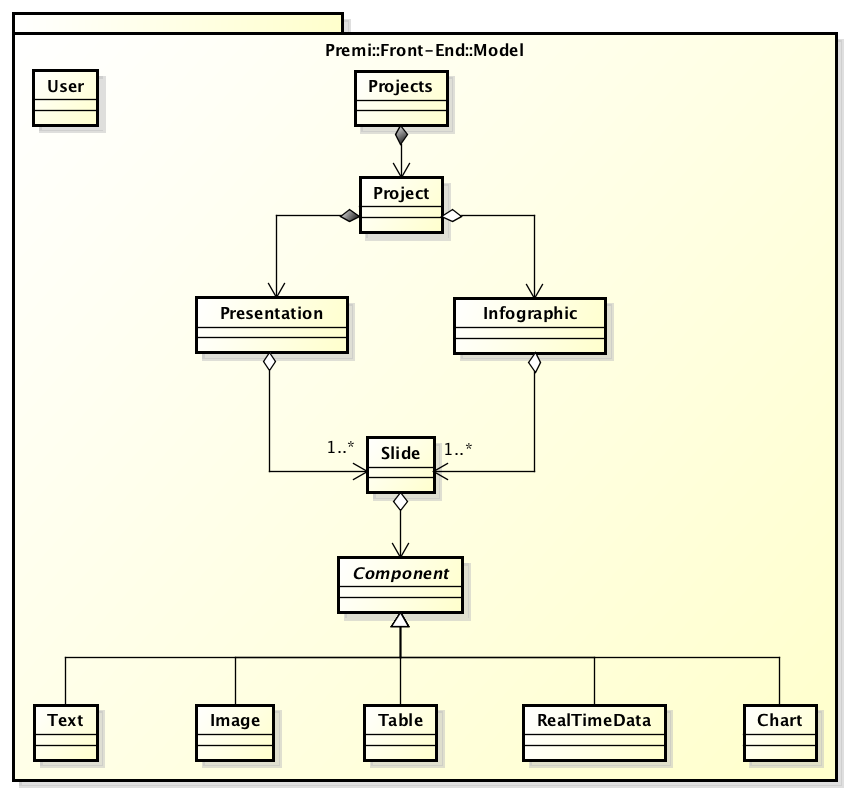
\includegraphics[width=0.7\linewidth]{img/premi_front_end_model}
	\caption[Premi::Front-End::Model]{Premi::Front-End::Model}
\end{figure}
Il package gestisce la memorizzazione delle informazioni dei dati utilizzati nel front-end e la loro logica. Al suo interno è presente una struttura di classi creata per ottimizzare il recupero e il salvataggio di dati anche con il rispettivo model del back-end.\\
Non è stato inserito un dettaglio di metodi ed attributi per quanto riguarda il front-end poiché è stato mantenuto identico a quello del back-end e si sarebbe trattata di una ridondanza che non avrebbe portato nessuna informazione aggiuntiva.